\chapwithtoc{Příloha 1}
\label{app:testing}

Tato příloha obsahuje podrobná data z~uživatelského testování. Obrázek~\ref{fig:priloha_1_1} obsahuje statistiky správně oanotovaných obrázků pro~oba testy. Navíc obsahuje seznam všech textů ve~kterých anotátoři správný obrázek neuhádli spolu se jménem dotyčného anotátora.

Obrázek~\ref{fig:priloha_1_2} obsahuje statistiky pro~každého z~anotátorů. Statistiky jsou jak celkové tak jednotlivé pro~všechny dvojice anotátorů, kteří spolu anotovali alespoň jeden stejný text. pro~každou dvojici anotátorů je uvedena matice $2\times2$ se statistikou shody a neshody anotátorů. z~této matice je pak spočítáno Cohenovo kappa pro~každou z~dvojic anotátorů.

\begin{figure}[h]
  \centering
  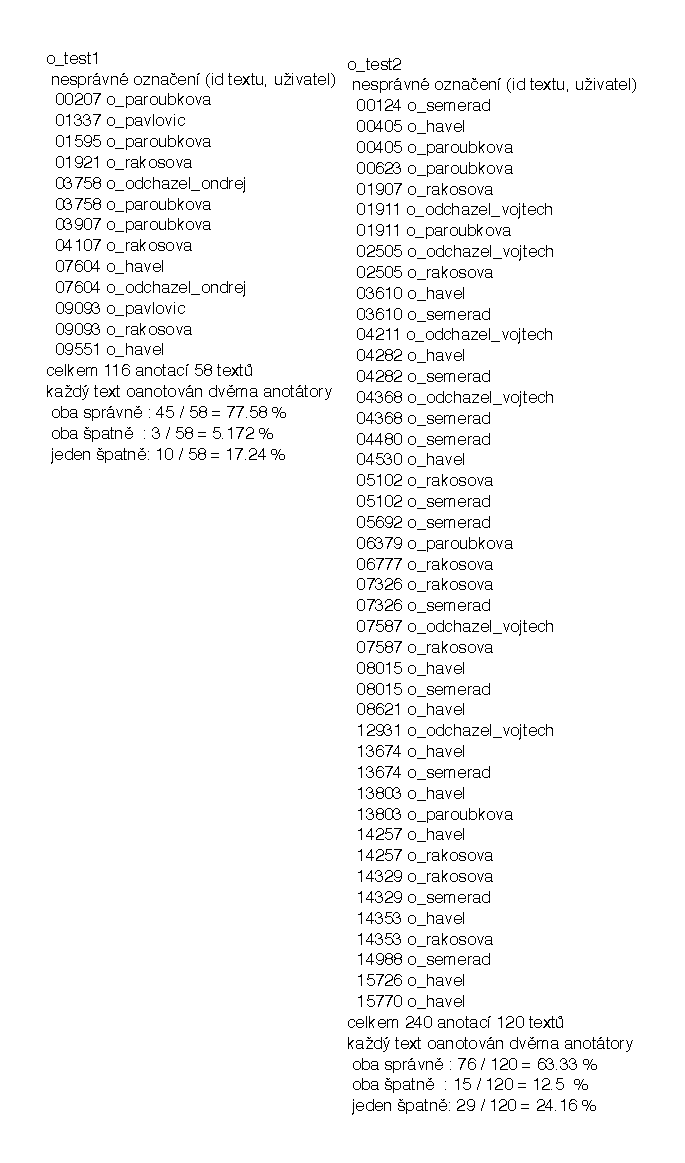
\includegraphics[height=8in]{priloha_1_1.eps}
  \caption{Výsledky textů a id textů se špatně detekovanými obrázky.}
  \label{fig:priloha_1_1}
\end{figure}


\begin{figure}[h]
  \centering
  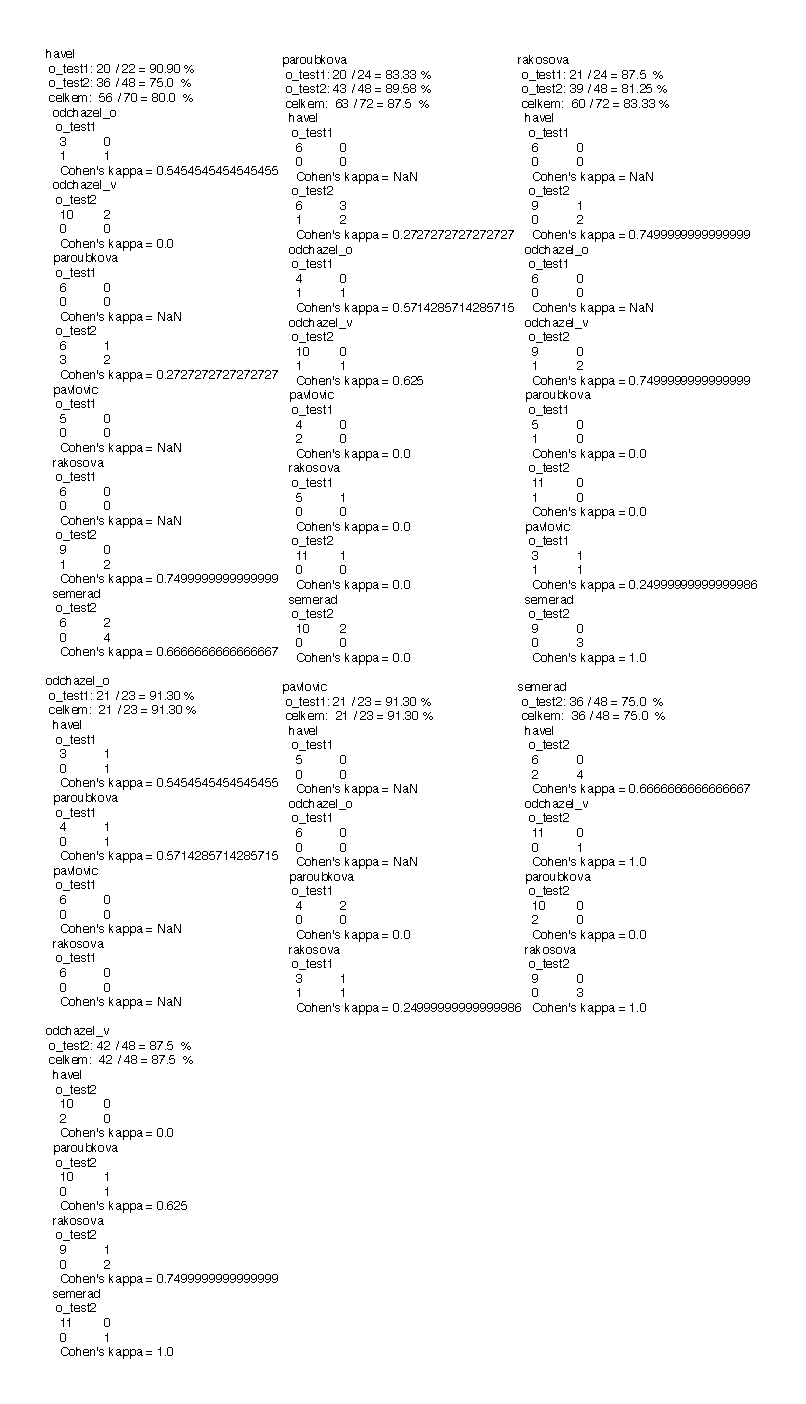
\includegraphics[height=8in]{priloha_1_2.eps}
  \caption{Výsledky textů a id textů se špatně detekovanými obrázky.}
  \label{fig:priloha_1_2}
\end{figure}

%\lstinputlisting[basicstyle=\ttfamily\scriptsize]{annotation_results.txt}